%نام و نام خانوادگی:
%شماره دانشجویی: 
\مسئله{SDD}
\پاسخ{
\\
\\
1.
\\
در این 
SDD
اگر علامت همراه دنباله اعداد + باشد ، ماکزیمم عدد موجود در رشته محاسبه می‌شود.
در غیر این صورت ( یعنی اگر علامت همراه رشته اعداد - باشد)
مینیمم عدد موجود در آن محاسبه می‌شود.

2.
\\
این SDD شامل دو صفت
sign
و 
val است.
sign
برای A
یک  attribute inherited است
زیرا A.sign
از parent خود در قاعده تولید محاسبه می‌شود.
در این قاعده تولید sign
برای Sign
یک
 attribute synthesized
است 
زیرا از روی مقدار خودش یا 
descendent
هایش
در قاعده تولید محاسبه می‌شود.
\\
attribute
دیگر یعنی val
نیز به همین دلیل یک 
attribute
synthesized
است.
\\
\\
3.
\\
\begin{figure}[htp]
    \centering
    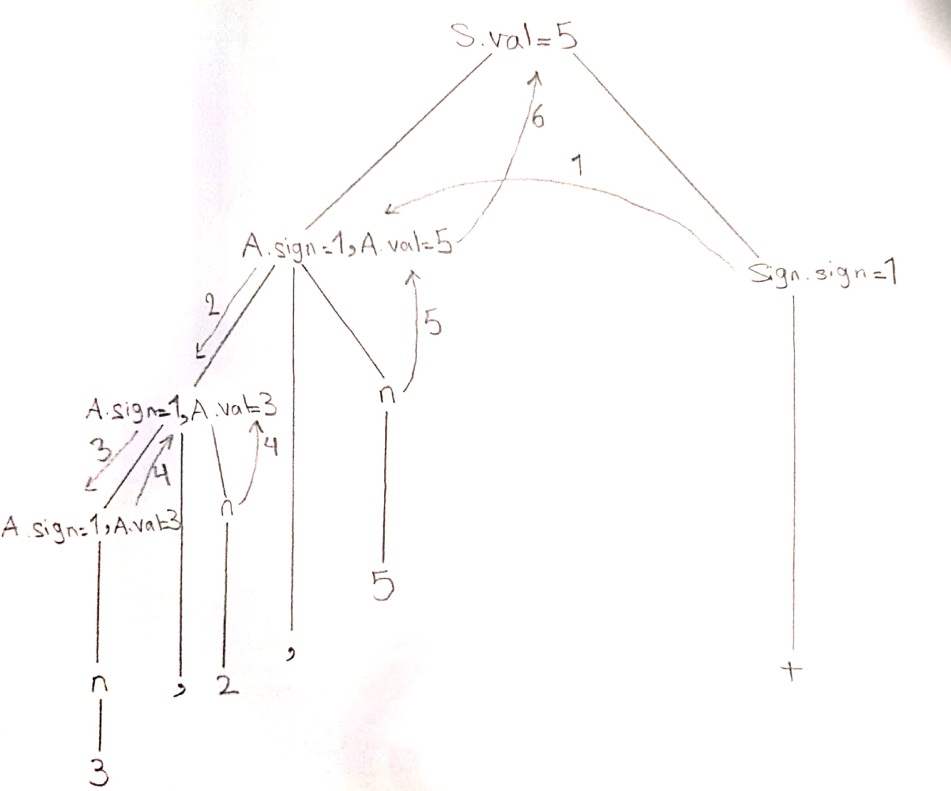
\includegraphics[width=12cm]{copm.png}
\end{figure}  



4.
\\
B و C هر دو nonterminal هستند:
\begin{latin}
\begin{enumerate}

    \item 
    S \rightarrow  B+ | S.val = B.val ; print(B.val)
    
    \item
	S \rightarrow C- | S.val= C.val , print(C.val)
	
    \item
    C \rightarrow n| C.val= value(n)
    
	\item
	B \rightarrow n | B.val=value(n)
	
	\item
	B \rightarrow B1,n | B.val= max(B1.val,value(n))
	
\end{enumerate}
\end{latin}

	
	

}